\section{Results}

\subsection{The estimator tracks true topic coverage}

On the Zipf mixtures, where every document's topic is known, coverage $1 - G$ at a radius of half the median pairwise distance of a pilot tracks the true topic mass coverage of the sample with Spearman $\rho = 0.968$ and a mean absolute error of 0.029, across 50 to 500 topics, two noise levels, three seeds and eleven sample sizes from 50 to 5{,}000. Good-Turing on the true labels, which the estimator does not see, reaches $\rho = 0.989$ and error 0.016. At smaller radii the agreement falls away ($\rho = 0.31$ at a tenth of the median distance). The radius matters, and the next result removes it as a free choice.

\subsection{The isolation rate collapses on $n r^{d}$}
\label{sec:collapse}

Table~\ref{tab:collapse} reports the one variable fit of Equation~\ref{eq:collapse} with $d$ fixed at its TwoNN estimate, over an $(n, r)$ grid of eleven sample sizes from 100 to 7{,}000 and twelve radii from the 5th to the 99th percentile of the pilot's nearest neighbour distances. On the three manifolds the fit explains 95\% to 97\% of the variance of $\log(-\log G)$, against 4\% to 6\% for $\log n$ alone and 64\% to 73\% for $\log r$ alone. On AskDocs, TIFU and the random tweet corpus it explains 95\% to 97\%. Fitted on cells with $n \le 1{,}000$ and tested on cells with $n$ up to 7{,}000, the law keeps $R^2$ of 0.93 to 0.96, and the isolation rate it predicts at $n = 7{,}000$ has a mean absolute error of 0.044 on AskDocs, 0.029 on TIFU and 0.051 on the tweets. Across seeds 42 to 44 on the forum corpora the out of sample $R^2$ is 0.950 (sd 0.019) on AskDocs and 0.954 (sd 0.004) on TIFU. Figure~\ref{fig:collapse} shows the surface against $n r^{d}$.

The fit with two regressors recovers the dimension without TwoNN. The ratio of the $\log r$ to the $\log n$ coefficient is 2.1, 4.4 and 7.3 on the manifolds of true dimension 2, 4 and 8, and 15.4 and 19.2 on AskDocs and TIFU against TwoNN values of 13.6 and 17.7. The exponent $b$ is below 1 everywhere: 0.60 to 0.75 on the Gaussian manifolds, whose density falls off from the centre, and 0.45 on AskDocs and TIFU. The stretched form is the rule.

\begin{table*}[t]
\centering
\small
\begin{tabular}{lrrrrrr}
\toprule
Corpus & $d$ (TwoNN) & $R^2$, $n r^{d}$ & $R^2$, $n$ only & $R^2$, $r$ only & out of sample $R^2$ & error at $n{=}7{,}000$ \\
\midrule
Manifold $d{=}2$ & 2.01 & 0.970 & 0.060 & 0.635 & 0.952 & 0.032 \\
Manifold $d{=}4$ & 4.21 & 0.954 & 0.044 & 0.666 & 0.924 & 0.056 \\
Manifold $d{=}8$ & 7.60 & 0.971 & 0.054 & 0.731 & 0.939 & 0.031 \\
AskDocs & 13.6 & 0.973 & 0.023 & 0.801 & 0.931 & 0.044 \\
TIFU & 17.7 & 0.972 & 0.041 & 0.826 & 0.956 & 0.029 \\
Tweets (random) & 14.5 & 0.946 & 0.033 & 0.863 & 0.939 & 0.051 \\
Trump & 9.2 & 0.811 & 0.000 & 0.731 & 0.636 & 0.064 \\
Zipf, 200 topics & 11.0 & 0.662 & 0.003 & 0.558 & 0.639 & 0.141 \\
\bottomrule
\end{tabular}
\caption{Collapse of the isolation surface. $R^2$ of $\log(-\log G)$ on $\log(n r^{d})$, on $\log n$ alone and on $\log r$ alone over all grid cells with $0.02 < G < 0.98$; out of sample $R^2$ and the mean absolute error of the predicted $G$ at $n = 7{,}000$ come from a fit on cells with $n \le 1{,}000$. Seed 42; seed means for the forum corpora are in the text.}
\label{tab:collapse}
\end{table*}

\begin{figure*}[t]
\centering
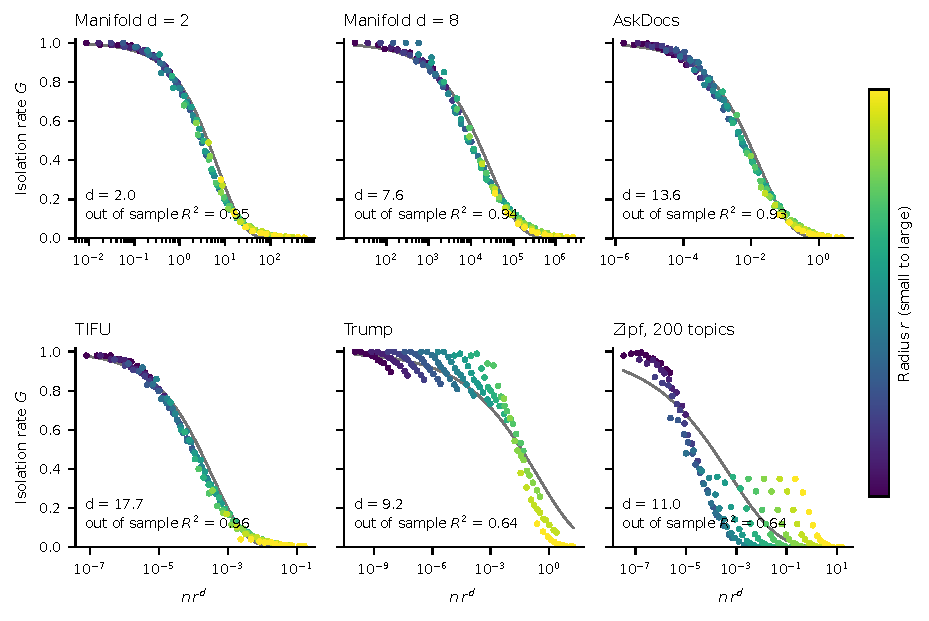
\includegraphics[width=\textwidth]{figures/collapse.pdf}
\caption{Isolation rate $G$ against $n r^{d}$ on a log scale, one panel per corpus, colour by radius $r$. Points from different radii fall on one curve where the law holds (AskDocs, TIFU, the manifolds) and separate where it fails (Trump, the Zipf mixture).}
\label{fig:collapse}
\end{figure*}

\subsection{Where the collapse fails, and why}

Trump and the Zipf mixture fail the fit (out of sample $R^2$ 0.64 for both, and 0.56 with sd 0.09 for Trump across seeds). In a 5{,}000-document sample of Trump, 3.4\% of documents have a near duplicate within cosine distance 0.02, against 0.0\% in AskDocs and TIFU, and the TwoNN dimension of its twenty $k$-means clusters runs from 2.0 to 16.2 (coefficient of variation 0.52, against 0.15 for AskDocs and 0.10 for TIFU). The clusters of dimension near 2 are slogans and the clusters near 16 are discussion. Removing the 266 near duplicates leaves the out of sample $R^2$ at 0.74, so the cause is the spread of local dimension and one global $d$ cannot describe both kinds of cluster. The Zipf mixture fails for the related reason of unequal topic mass, with no duplicates. The $R^2$ of the collapse fit is therefore a diagnostic: a corpus that collapses has one dimension and one sample size formula, and a corpus that does not needs a mixture.

\subsection{The finite population correction}

Table~\ref{tab:fpc} compares $G$ and $G\,(1 - n/N)$ with the true missing mass $M$ of the finite corpus over four corpora (AskDocs, Trump, TIFU and the Zipf mixture), six sample sizes from 100 to 5{,}000 and six radii, 144 cells. Uncorrected, $G$ has a mean absolute error of 0.068 and a maximum of 0.42, reached at $n = 5{,}000$ of $N = 10{,}000$, where $G$ is twice $M$. Corrected, the mean error is 0.015, the maximum 0.11 and the Spearman correlation 0.996. Across the three seeds on the forum corpora the corrected error is 0.010 on AskDocs, 0.013 on TIFU and 0.009 on Trump, so the correction holds on the corpus that fails the collapse as well.

\begin{table}[t]
\centering
\small
\begin{tabular}{rrrr}
\toprule
$n$ & $M$ (true) & $G$ & $G\,(1 - n/N)$ \\
\midrule
100 & 0.729 & 0.749 & 0.743 \\
200 & 0.665 & 0.684 & 0.672 \\
500 & 0.565 & 0.600 & 0.574 \\
1{,}000 & 0.479 & 0.534 & 0.486 \\
2{,}000 & 0.378 & 0.463 & 0.380 \\
5{,}000 & 0.211 & 0.384 & 0.212 \\
\bottomrule
\end{tabular}
\caption{Missing mass of the finite corpus, mean over four corpora and six radii at each $n$. $N$ is 10{,}000 for the three forum corpora and 20{,}000 for the Zipf mixture.}
\label{tab:fpc}
\end{table}

\subsection{Theme coverage is a question about a partition}
\label{sec:themes}

With thirty themes per corpus, the share of theme mass present in a sample is the same in all eight forum and census corpora at every $n$: 0.58 to 0.65 at $n = 25$, 0.82 to 0.86 at $n = 50$, 0.94 to 0.98 at $n = 100$ and 0.99 to 1.00 at $n = 200$ (Figure~\ref{fig:themes}). Equation~\ref{eq:gt}, evaluated on each corpus's theme masses, reproduces these values with a mean absolute error of 0.005. Over the same samples, coverage at a fixed resolution ($1 - G$ at $r = 0.34$) runs from 0.003 on AskDocs to 0.77 on citizens at $n = 25$. A quantity that is the same everywhere cannot be ordered by one that differs tenfold, and the Spearman correlation across corpora between the two is accordingly near zero at every $n$.

The language model's enumeration behaves as the partition says it should. Within each corpus the mass of themes Gemma~4 reports present rises with $n$ along the label coverage curve (Spearman $+1.00$ in seven corpora and $+0.90$ in TIFU), and its precision against the label truth rises from 0.73 at $n = 25$ to 0.98 at $n = 400$. Merging the eight inventories into one shared taxonomy at four merge radii (42 to 187 shared themes) opens up differences across corpora, and those differences are predicted by the shared masses through Equation~\ref{eq:gt} (Spearman $+0.93$ to $+1.00$) and not by $G$ at any fixed radius ($+0.31$, $+0.21$, $+0.38$ and $-0.40$ at $n = 50$ for the four merges). Appendix~\ref{app:shared} gives the full table.

The two questions are therefore different functionals of the same geometry. Coverage of a partition is set by the partition's mass vector. The missing mass at resolution $r$ is set by the local geometry at scale $r$, and the two coincide only when the partition's cells are balls of radius $r$, which thematic clusters are not. A user who asks ``have I seen every theme'' should use Equation~\ref{eq:gt} with the theme masses, which a pilot inventory supplies. A user who asks ``is every document within $r$ of something I have read'' should use $G$, the collapse law and Equation~\ref{eq:nstar}.

\begin{figure}[t]
\centering
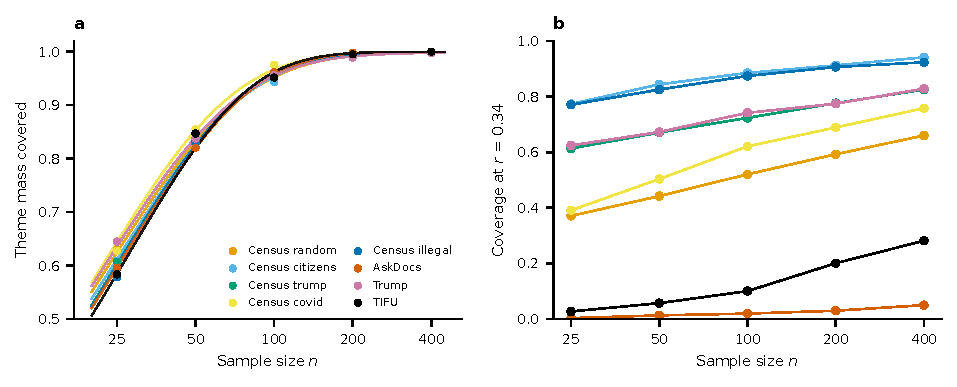
\includegraphics[width=\columnwidth]{figures/themes.pdf}
\caption{Share of theme mass present in a sample against $n$, eight corpora with thirty themes each (points), and the Good-Turing expectation of Equation~\ref{eq:gt} from each corpus's theme masses (lines).}
\label{fig:themes}
\end{figure}

\subsection{Truth Social and Bluesky}

\textcolor{red}{[Pending: the two 50{,}000-post samples are being embedded. This subsection will report their $d$, collapse $R^2$ and finite population correction once the run lands.]}
